\documentclass[12pt]{exam}

\newcommand{\ds}{\ensuremath{\displaystyle}}

\usepackage{amsmath,amsfonts, amsthm}
\usepackage{multicol}
\usepackage{multirow}
\usepackage{harpoon}
\renewcommand{\arraystretch}{1.5}

\newcommand{\harpvec}[1]{\overrightharp{\ensuremath{\mathbf{#1}}}}
\newcommand{\vect}[1]{\harpvec{#1}}
\newcommand{\<}{\langle}
\renewcommand{\>}{\rangle}

% ref: http://pgfplots.sourceforge.net/gallery.html
% ref: http://tex.stackexchange.com/a/74575/79754
\usepackage{pgfplots}% This uses tikz
\pgfplotsset{compat=newest}% use newest version
\tikzset{LineStyle/.style={smooth, ultra thick, samples=400}}

% \printanswers

\begin{document}

\begin{center}
\fbox{\fbox{\parbox{5.5in}{\centering
MATH 1121 - Fall 2015 - Dr. Clontz - Test 1
}}}
\end{center}
\vspace{0.1in}
\makebox[\textwidth]{
  Name:\enspace\hrulefill\hrulefill\hrulefill\space
  Section:\enspace\hrulefill\space
}

\vspace{12pt}

\begin{itemize}
  \item This test is worth 250 points toward your overall grade.
        Each problem is labeled with its value toward this total.
  \item On multiple choice problems, you do not need to show your work. No
        partial credit will be given.
  \item On full response problems, show all of your work and give a
        complete solution. When in doubt, don't skip any steps. Partial
        credit will be given at the discretion of the instructor.
  \item This exam is open notes, provided that these notes are completely
        in your own handwriting. The professor may take up notes you use
        with your test and return them after the test is graded.
  \item Tests submitted after the end of 70 minutes will be deducted 25 points,
        with 25 more points deducted every following minute.
\end{itemize}

\newpage

\begin{center}
  \textbf{Multiple Choice (150 points total)}
\end{center}

\begin{questions}

\setcounter{question}{0}
\question[15]
Two endpoints of a line segment are \((-1,-1)\) and \((-1,3)\).
What must the \(y\)-coordinate of the line segment's midpoint be?


\begin{checkboxes}
\choice \(-1\)
\choice \(0\)
\choice \(1\)
\choice \(3\)
\choice None of these
\end{checkboxes}

\vfill

\question[15]
What is the distance between the points with coordinates \((3,-2)\)
and \((0,-6)\)?

\begin{checkboxes}
\choice \(5\)
\choice \(\sqrt{7}\)
\choice \(\sqrt{35}\)
\choice \(25\)
\choice None of these
\end{checkboxes}

\vfill

\question[15]
Consider the lines with equations \(y=\frac{1}{2}x+5\) and \(2x+y+3=0\).
Which of these statements is true?

\begin{checkboxes}
\choice The lines are parallel, but not perpendicular.
\choice The lines are perpendicular, but not parallel.
\choice The lines are both parallel and perpendicular.
\choice The lines are neither parallel nor perpendicular.
\choice None of these.
\end{checkboxes}

\vfill
\newpage

\question[15]
Which of the following plots corresponds to the circle with the following equation?
\[(x+2)^2+(y-3)^2=16\]

\begin{multicols}{2}
\begin{checkboxes}

  \choice
    \fbox{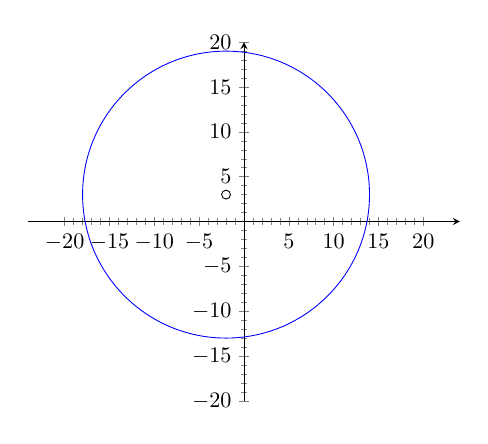
\begin{tikzpicture}[scale=0.8]
    \begin{axis}[
        axis equal,
        xmin=-20,
        xmax=20,
        xtick={-20,-15,...,20},
        ymin=-20,
        ymax=20,
        ytick={-20,-15,...,20},
        minor tick num=4,
        axis lines=middle,
    ]
      \draw[blue] \pgfextra{
        \pgfpathellipse{\pgfplotspointaxisxy{-2}{3}}
            {\pgfplotspointaxisdirectionxy{16}{0}}
            {\pgfplotspointaxisdirectionxy{0}{16}}
        };
      \addplot [only marks,mark=o] coordinates { (-2,3) } ;
    \end{axis}
    \end{tikzpicture}}

  \choice
    \fbox{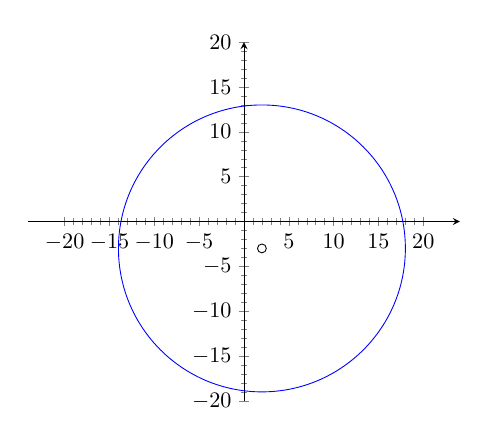
\begin{tikzpicture}[scale=0.8]
    \begin{axis}[
        axis equal,
        xmin=-20,
        xmax=20,
        xtick={-20,-15,...,20},
        ymin=-20,
        ymax=20,
        ytick={-20,-15,...,20},
        minor tick num=4,
        axis lines=middle,
    ]
      \draw[blue] \pgfextra{
        \pgfpathellipse{\pgfplotspointaxisxy{2}{-3}}
            {\pgfplotspointaxisdirectionxy{16}{0}}
            {\pgfplotspointaxisdirectionxy{0}{16}}
        };
      \addplot [only marks,mark=o] coordinates { (2,-3) } ;
    \end{axis}
    \end{tikzpicture}}

  \columnbreak

  \choice
    \fbox{\begin{tikzpicture}[scale=0.8]
    \begin{axis}[
        axis equal,
        xmin=-11,
        xmax=11,
        xtick={-10,-5,0,5,10},
        ymin=-11,
        ymax=11,
        ytick={-10,-5,0,5,10},
        minor tick num=4,
        axis lines=middle,
    ]
      \draw[blue] \pgfextra{
        \pgfpathellipse{\pgfplotspointaxisxy{-2}{3}}
            {\pgfplotspointaxisdirectionxy{4}{0}}
            {\pgfplotspointaxisdirectionxy{0}{4}}
        };
      \addplot [only marks,mark=o] coordinates { (-2,3) } ;
    \end{axis}
    \end{tikzpicture}}

  \choice
    \fbox{\begin{tikzpicture}[scale=0.8]
    \begin{axis}[
        axis equal,
        xmin=-11,
        xmax=11,
        xtick={-10,-5,0,5,10},
        ymin=-11,
        ymax=11,
        ytick={-10,-5,0,5,10},
        minor tick num=4,
        axis lines=middle,
    ]
      \draw[blue] \pgfextra{
        \pgfpathellipse{\pgfplotspointaxisxy{2}{-3}}
            {\pgfplotspointaxisdirectionxy{4}{0}}
            {\pgfplotspointaxisdirectionxy{0}{4}}
        };
      \addplot [only marks,mark=o] coordinates { (2,-3) } ;
    \end{axis}
    \end{tikzpicture}}

  \choice None of these.

\end{checkboxes}
\end{multicols}

\vfill

\question[15]
Which of the following equations corresponds to the parabola sketched here?

\begin{center}
    \fbox{\begin{tikzpicture}[scale=0.8]
    \begin{axis}[
        axis equal,
        xmin=-11,
        xmax=11,
        xtick={-10,-5,0,5,10},
        ymin=-11,
        ymax=11,
        ytick={-10,-5,0,5,10},
        minor tick num=4,
        axis lines=middle,
    ]
      \addplot[blue,samples=100,domain=-10:10] ({-x^2/12}, {x});
      \addplot[dashed,samples=100,domain=-10:10] ({3}, {x});
      \addplot[only marks,mark=o] coordinates { (-3,0) } ;
    \end{axis}
    \end{tikzpicture}}
\end{center}

\begin{multicols}{2}
\begin{checkboxes}
  \choice \(y=\frac{x^2}{12}\)
  \choice \(x=\frac{y^2}{12}\)
  \choice \(y=-\frac{x^2}{12}\)
  \choice \(x=-\frac{y^2}{12}\)
  \choice None of these.
\end{checkboxes}
\end{multicols}

\vfill
\newpage


\question[15]
Consider the ellipse with equation \(\frac{x^2}{25}+\frac{y^2}{9}=1\).
Every point on this ellipse must be equidistant from which pair of points?

\begin{checkboxes}
  \choice \((4,0)\) and \((-4,0)\)
  \choice \((0,4)\) and \((0,-4)\)
  \choice \((34,0)\) and \((-34,0)\)
  \choice \((0,34)\) and \((0,-34)\)
  \choice None of these.
\end{checkboxes}

\vfill

\question[15]
Which of these is an equation of the hyperbola centered at the origin
with a focus at \((0,\sqrt{13})\) and vertex at \((0,-2)\)?

\begin{checkboxes}
  \choice \(\frac{y^2}{13}-\frac{x^2}{4}=1\)
  \choice \(\frac{y^2}{13}-\frac{x^2}{9}=1\)
  \choice \(\frac{y^2}{4}-\frac{x^2}{9}=1\)
  \choice \(\frac{y^2}{4}-\frac{x^2}{13}=1\)
  \choice None of these.
\end{checkboxes}

\vfill

\question[15]
Describe the translation of the graph with equation \((x-2)^2=4(y+1)\)
in comparison to the graph with equation \(x^2=4y\).

\begin{checkboxes}
  \choice \(2\) units right and \(1\) unit down.
  \choice \(2\) units left and \(1\) unit down.
  \choice \(2\) units right and \(1\) unit up.
  \choice \(2\) units up and \(1\) unit left.
  \choice None of these.
\end{checkboxes}

\vfill
\newpage

\question[15]
Which of these is a simplification of the following algebraic function?
\[
  f(x)
    =
  \frac{
    (3x+1)(2x^{-1/2})-2x^{1/2}(3)
  }{
    (3x+1)^2
  }
\]

\begin{checkboxes}
  \choice \(\ds f(x)=\frac{2x-1}{(6x+\sqrt{x})^2}\)
  \choice \(\ds f(x)=\frac{6x-3}{x^{1/2}(3x+1)^2}\)
  \choice \(\ds f(x)=\frac{x^{1/2}}{3x+1}\)
  \choice \(\ds f(x)=\frac{2x}{x^{1/2}(3x+1)^{1/2}}\)
  \choice None of these.
\end{checkboxes}

\vfill

\question[15]
Which of these is the graph of the function \(g(x)=\frac{4}{x-1}\)?

\begin{multicols}{2}
\begin{checkboxes}
  \choice
    \fbox{\begin{tikzpicture}[scale=0.8]
    \begin{axis}[
        axis equal,
        xmin=-11,
        xmax=11,
        xtick={-10,-5,0,5,10},
        ymin=-11,
        ymax=11,
        ytick={-10,-5,0,5,10},
        minor tick num=4,
        axis lines=middle,
    ]
      \addplot[blue,domain=-10:0.9] ({x},{(4)/(x-1)});
      \addplot[blue,domain=1.1:10] ({x},{(4)/(x-1)});
      \addplot[dashed,domain=-10:10] ({1},{x});
    \end{axis}
    \end{tikzpicture}}

  \choice
    \fbox{\begin{tikzpicture}[scale=0.8]
    \begin{axis}[
        axis equal,
        xmin=-11,
        xmax=11,
        xtick={-10,-5,0,5,10},
        ymin=-11,
        ymax=11,
        ytick={-10,-5,0,5,10},
        minor tick num=4,
        axis lines=middle,
    ]
      \addplot[blue,domain=-3:3,samples=100] ({2*x^3},{4*x});
    \end{axis}
    \end{tikzpicture}}

  \choice
    \fbox{\begin{tikzpicture}[scale=0.8]
    \begin{axis}[
        axis equal,
        xmin=-11,
        xmax=11,
        xtick={-10,-5,0,5,10},
        ymin=-11,
        ymax=11,
        ytick={-10,-5,0,5,10},
        minor tick num=4,
        axis lines=middle,
    ]
      \addplot[blue,domain=-10:3,samples=100] ({x+1},{4^x});
    \end{axis}
    \end{tikzpicture}}

  \choice
    \fbox{\begin{tikzpicture}[scale=0.8]
    \begin{axis}[
        axis equal,
        xmin=-11,
        xmax=11,
        xtick={-10,-5,0,5,10},
        ymin=-11,
        ymax=11,
        ytick={-10,-5,0,5,10},
        minor tick num=4,
        axis lines=middle,
    ]
      \addplot[blue,domain=-10:10,samples=100] ({x},{2*sin(90*x)});
    \end{axis}
    \end{tikzpicture}}


  \choice None of these.
\end{checkboxes}
\end{multicols}




\end{questions}





\vfill
\newpage






\begin{center}
  \textbf{Full Response (100 points total)}
\end{center}

\begin{questions}

\setcounter{question}{10}

\question[20]
  Show how to find an equation for the line passing through
  the point \((3,-2)\) with slope \(-2\), and then sketch it on the given
  coordinate plane.

  \vfill


  \begin{center}
    \begin{tikzpicture}[scale=2]
    \begin{axis}[
        axis equal,
        xmin=-7,
        xmax=7,
        xtick={-6,-3,...,6},
        ymin=-7,
        ymax=7,
        ytick={-6,-3,...,6},
        minor tick num=2,
        axis lines=middle,
    ]
    \end{axis}
    \end{tikzpicture}
  \end{center}


\newpage

\question[20]
  Give the equation of the below graph, and add its foci to the graph.

  \begin{center}
    \begin{tikzpicture}[scale=2]
    \begin{axis}[
        axis equal,
        xmin=-20,
        xmax=20,
        xtick={-20,-15,...,20},
        ymin=-20,
        ymax=20,
        ytick={-20,-15,...,20},
        minor tick num=4,
        axis lines=middle,
    ]
      \draw[blue] \pgfextra{
        \pgfpathellipse{\pgfplotspointaxisxy{0}{0}}
            {\pgfplotspointaxisdirectionxy{5}{0}}
            {\pgfplotspointaxisdirectionxy{0}{13}}
        };
    \end{axis}
    \end{tikzpicture}
  \end{center}


\newpage

\question[20]
  Sketch the hyperbola centered at the origin with vertex \((-3,0)\) and
  focus \((-5,0)\), including its asymptotes and other focus.

  \begin{center}
    \begin{tikzpicture}[scale=2]
    \begin{axis}[
        axis equal,
        xmin=-11,
        xmax=11,
        xtick={-10,-5,...,10},
        ymin=-11,
        ymax=11,
        ytick={-10,-5,...,10},
        minor tick num=4,
        axis lines=middle,
    ]
    \end{axis}
    \end{tikzpicture}
  \end{center}


\newpage

\question[20]
  Use algebra to manipulate \(x^2-6x+8y+17=0\) to get the equation of
  a translated parabola. (You do not need to sketch
  the graph. Hint: the parabola has its vertex at \((3,-1)\).)

\newpage

\question[20]
  Give a simplified expression for the composition \((f\circ g)(x)\) given
  \(f(x)=x^2-3x\) and \(g(x)=2x-1\).

\end{questions}

\end{document}